\section{Abstrakte simpliziale Komplexe}

\begin{thDef}%
    [Abstrakter simplizialer Komplex]
    Ist $V$ eine Menge und $K\subset\pot{V}$, so dass alle Elemente von $K$
    endliche Mächtigkeit haben, so ist $(V,K)$ ein \emph{abstrakter simplizialer
    Komplex}, falls zusätzlich gilt:
    \[ \forall\,F\in K 
        \;\forall\, F'\subset F \colon\; F'\in K
    . \]
    Ein Element $F\in K$ nennen wir \emph{(abstraktes) Simplex} und die
    \emph{Dimension von $F$} ist gegeben durch $\dim(F) \defeq
    \abs{F}-1$.
    Die \emph{Dimension von $K$} ist wie folgt definiert:
    \[ \dim(K) \defeq \max_{F\in K}\,\dim(F)  \;\in\N\cup\{\infty\}  . \]
    Ist $\abs{V}$ endlich, so sprechen wir von einem \emph{endlichen
    simplizialen Komplex}. Ist $(V',K')$ ein simplizialer Komplex mit 
    $V'\subset V$ und $K'\subset K$, so nennen wir diesen einen
    \emph{Teilkomplex von $(V,K)$}.
\end{thDef}

\begin{thAufgabe}
    Überlegen Sie, wie man Graphen als abstrakte simpliziale Komplexe auffassen kann.
\end{thAufgabe}

Anstatt des Paars $(V,K)$ notieren wir oft nur noch $K$ und nehmen $V=\bigcup K$
an. Außerdem können wir aus jedem geometrischen
simplizialen Komplex~$\Delta$ einen abstrakten gewinnen, indem wir wie folgt
vorgehen: Sei $V$ die Menge aller Ecken von Simplizes aus $\Delta$ und $K$ wie folgt
gegeben:
\[ K \defeq \bigl\{ V_\sigma 
    \Mid V_\sigma \text{ ist Eckenmenge eines Simplex $\sigma\in\Delta$} \bigr\}
. \]
Dann ist $(V,K)$ klarerweise ein abstrakter simplizialer Komplex und wir nennen
$\Delta$ eine \emph{geometrische Realisierung von $K$}.  Das Polyeder
$\polyeder\Delta$ bezeichnen wir dann auch als ein \emph{Polyeder von $K$}. 
\begin{center}
    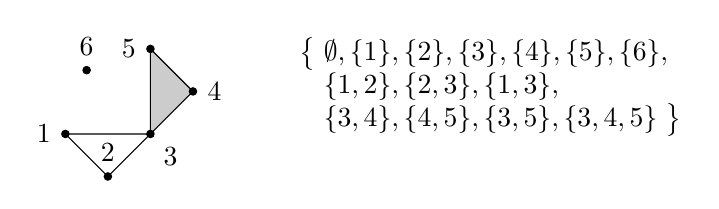
\begin{tikzpicture}[%
        scale=0.6,
        mypoint/.style={shape=circle, inner sep=1.1pt, color=black, fill}
    ]
        \begin{scope}[scale=0.90]
            \coordinate (1) at (0,0);
            \coordinate (2) at (1,-1);
            \coordinate (3) at (2,0);
            \coordinate (4) at (3,1);
            \coordinate (5) at (2,2);
            \coordinate (6) at (0.5,1.5);
            
            \draw (1) -- (2) -- (3) -- cycle;
            \draw [fill=black!20] (3) -- (4) -- (5) -- cycle;
            
            \foreach \n/\ang in 
                {1/left,2/above,3/below right,4/right,5/left,6/above}
                \node [mypoint,label=\ang:$\n$] at (\n) {};
        \end{scope}

        \node [align=left] at (9,1) {%
            $\displaystyle
            \bigl\{\; \emptyset, \{1\}, \{2\}, \{3\}, \{4\}, \{5\}, \{6\},$    \\
            $\displaystyle\hphantom{\bigl\{\;}
                    \{1,2\}, \{2,3\}, \{1,3\},$                     \\
            $\displaystyle\hphantom{\bigl\{\;}
                    \{3,4\}, \{4,5\}, \{3,5\}, \{3,4,5\}
            \;\bigr\}$%
        };
    \end{tikzpicture}
    \\
    \footnotesize
    Geometrische Realisierung (links) und zugehöriger abstrakter
    simplizialer Komplex (rechts)
\end{center}

\begin{thSatz}%
    [Maximal nötige Dimension einer geometrischer Realisierung]
    \label{asc:geomrealization}
    %
    Sei $K$ ein endlicher simplizialer Komplex der Dimension~$d\in\N$.
    Dann besitzt $K$ eine geometrische Realisierung im $\R^{2d+1}$.
\end{thSatz}

Wir können aus jeder (endlichen) partiell geordneten Menge einen (endlichen)
simplizialen Komplex bilden und umgekehrt.
Folgende Definitionen legen fest, wie wir dies tun wollen:

\begin{thDef}[Ordnungskomplex]
    Sei $(P,\leq)$ eine partiell geordnete Menge. Dann definiert
    $\bigl\{ \{x_1,\ldots,x_k\} \subset P \cMid[\;]\big 
        k\in\N,\; x_1\leq \dots \leq x_k \bigr\}$
    den \emph{Ordnungskomplex $\Delta(P)$  von $P$}.
\end{thDef}

\begin{thDef}[Partielle Ordnung auf simplizialem Komplex]
    Ist $K$ ein simplizialer Komplex, so wird
    $K\setminus\{\emptyset\}$ durch die Inklusionsrelation~\enquote{$\subset$} 
    partiell geordnet. Wir bezeichnen diese zu $K$ assoziierte 
    partiell geordnete Menge mit $P(K)$.
\end{thDef}

\begin{thAufgabe}
    Sei $T \defeq \{1,2,3,4\}$ durch die
    Teilerrelation~\enquote{$\mkern1mu|\mkern2mu$} partiell geordnet.
    Verdeutlichen Sie sich die Konzepte der beiden vorangehenden Definitionen,
    indem Sie zunächst $K\defeq\Delta(T)$ bilden und eine geometrische Realisierung
    skizzieren. Bilden Sie anschließend $P(K)$ ($\rightsquigarrow$
    Hasse-Diagramm) und überlegen Sie sich anschließend, wie eine geometrische
    Realisierung von $\Delta\bigl(P(K)\bigr)$ aussieht.
\end{thAufgabe}
